\documentclass[12pt]{article}
\usepackage[top=1in, bottom=1in, left=1in, right=1in]{geometry}

\usepackage{setspace}
\onehalfspacing

\usepackage{amssymb}
%% The amsthm package provides extended theorem environments
\usepackage{amsthm}
\usepackage{epsfig}
\usepackage{times}
\renewcommand{\ttdefault}{cmtt}
\usepackage{amsmath}
\usepackage{graphicx} % for graphics files

% Draw figures yourself
\usepackage{tikz} 

% writing elements
\usepackage{mhchem}

% The float package HAS to load before hyperref
\usepackage{float} % for psuedocode formatting
\usepackage{xspace}

% from Denovo Methods Manual
\usepackage{mathrsfs}
\usepackage[mathcal]{euscript}
\usepackage{color}
\usepackage{array}

\usepackage[pdftex]{hyperref}
\usepackage[parfill]{parskip}

% math syntax
\newcommand{\nth}{n\ensuremath{^{\text{th}}} }
\newcommand{\ve}[1]{\ensuremath{\mathbf{#1}}}
\newcommand{\Macro}{\ensuremath{\Sigma}}
\newcommand{\rvec}{\ensuremath{\vec{r}}}
\newcommand{\omvec}{\ensuremath{\hat{\Omega}}}
\newcommand{\vOmega}{\ensuremath{\hat{\Omega}}}
%---------------------------------------------------------------------------
%---------------------------------------------------------------------------
\begin{document}
\begin{center}
{\bf NE 155/255, Fall 2019\\
Transport Equation and Boundary Conditions\\
September 16, 2019}
\end{center}

\setlength{\unitlength}{1in}
\begin{picture}(6,.1) 
\put(0,0) {\line(1,0){6.25}}         
\end{picture}

\subsection*{Transport Equation (cont'd.)}

In order to build the transport equation, we sum the terms we derived previously with
appropriate signs for loss and gain, to the overall rate of change. Letting
$\triangle \beta$ approach a differential element and canceling it, we obtain

\begin{align}
\frac{\partial n}{\partial t} =&
-\left[\frac{\partial (\dot x n)}{\partial x} +
\frac{\partial (\dot y n)}{\partial y}+\frac{\partial (\dot z n)}{\partial z} +
\frac{\partial (\dot E n)}{\partial E}+
\frac{\partial (\dot \theta n)}{\partial \theta}+
\frac{\partial (\dot \varphi n)}{\partial \varphi}\right] 
\\ & \quad - v\Sigma_a(\rvec,E)n \nonumber
\\& \quad\quad\quad   + 
\int_0^{\infty}\int_{4\pi}
v'\Sigma_s(\rvec, E'\rightarrow E,\omvec'\rightarrow\omvec)
n(\rvec,E',\omvec',t) d\omvec'dE'\nonumber 
\\& \quad\quad\quad\quad\quad\quad -
\int_0^{\infty}\int_{4\pi}v
\Sigma_s(\rvec, E\rightarrow E',\omvec\rightarrow\omvec')
n(\rvec,E,\omvec,t) d\omvec'dE'\nonumber
\\& \quad\quad\quad\quad\quad\quad\quad\quad\quad
+S(\rvec,E,\omvec,t),\nonumber
\end{align}

where $n = n(\rvec,E,\omvec,t)$. Since particles travel in a straight line
between collisions, \linebreak
$\dot \theta = \dot \varphi = 0$. Furthermore, $\dot E = 0$ because particles 
stream with no change in energy. Finally, performing the outscattering 
integral:

\begin{align}
&\frac{1}{v}\frac{\partial \psi}{\partial t}(\rvec,E,\omvec,t) +
\omvec\cdot  \nabla \psi(\rvec,E,\omvec,t) +
\Sigma_t(\rvec,E)\psi(\rvec,E,\omvec,t)
\\& \quad =
\int_0^{\infty}\int_{4\pi}
\Sigma_s(\rvec, E'\rightarrow E,\omvec'\rightarrow\omvec)
\psi(\rvec,E',\omvec',t)d\omvec'dE'+S(\rvec, E, \omvec,t) \nonumber.
\end{align}

We can easily generalize this equation to include nuclear fission.
To do that, we must revisit our treatment of $\Sigma_a$; there are two main 
processes responsible for the absorption of particles in the system:
\textit{radiative capture} and \textit{nuclear fission} (note that we're 
ignoring (n,xn) reactions for the time being). Now, we define

\begin{align*}
\Sigma_\gamma(\rvec,E)d\beta = \textrm{probability of capture}
\end{align*}
and
\begin{align*}
\Sigma_f(\rvec,E)d\beta = \textrm{probability of a fission event},
\end{align*}
such that
\begin{align*}
\Sigma_a(\rvec,E) = \Sigma_\gamma(\rvec,E) + \Sigma_f(\rvec,E)\,.
\end{align*}

While a captured neutron is simply removed from the system, a neutron with 
energy $E$ that induces a fission event causes the target nucleus to split 
into two smaller daughter nuclei, and 

\begin{align*}
\nu(E) = \textrm{the mean number of fission neutrons that are released}.
\end{align*}

Of this number, $\nu(E)[1-M(E)]$ are \textit{prompt} fission neutrons (being 
emitted within $10^{-15}$ seconds of the fission event). These fission 
neutrons are emitted isotropically, with an energy distribution given by the 
fission spectrum $\chi_p(E)$. Also, $\nu(E)M(E)$ \textit{delayed} fission 
neutrons (being released roughly 0.1 to 60 seconds after the fission event) 
are created; a delayed neutron is produced when a radioactive daughter nucleus 
undergoes a radioactive decay process in which a neutron is emitted. 

Assuming (for simplicity) that the number of delayed neutrons emitted by 
fission is very small [$M(E)<<1$], we can neglect the delayed neutron terms 
and rewrite the transport equation as

\begin{align}
&\underbrace{\frac{1}{v}\frac{\partial \psi}{\partial t}(\rvec,E,\omvec,t)}_
            {\text{time rate of change}} + 
\underbrace{\omvec\cdot  \nabla \psi(\rvec,E,\omvec,t)}_
           {\text{streaming loss rate}} +
 \underbrace{\Sigma_t(\rvec,E)\psi(\rvec,E,\omvec,t) }_
            {\text{total interaction loss rate}}
\\& \quad\quad\quad\quad =
\underbrace{\int_0^{\infty}\int_{4\pi}
            \Sigma_s(\rvec, E'\rightarrow E,\omvec'\rightarrow\omvec)
            \psi(\rvec,E',\omvec',t)d\omvec'dE'}_
           {\text{in scattering source rate}}\nonumber
\\&\quad\quad\quad\quad\quad\quad +
\underbrace{\frac{\chi_p(E)}{4\pi}\int_0^{\infty}
            \int_{4\pi}\nu(E')\Sigma_f(\rvec,E')
            \psi(\rvec,E',\omvec',t)d\omvec'dE'}_
           {\text{fission source rate}}\nonumber
\\&\quad\quad\quad\quad\quad\quad\quad\quad+
\underbrace{S(\rvec, E, \omvec,t)}_{\text{external source rate}} \nonumber.
\end{align}   
   
\subsection*{Boundary and Initial Conditions}

These equations require both spatial and temporal boundary conditions.
\textit{Assuming that the physical system of interest is nonreentrant}
(convex) and characterized by a volume $V$, it is sufficient to specify the 
flux of particles at all points of the bounding surface of the system in the 
incoming directions. This implies

\begin{align*}
\psi(\rvec_s, E,\omvec,t) &=
\psi_b(\rvec_s,E,\omvec,t)\,, \hspace{0.5 cm} \textbf{n} \cdot \omvec <0,
\end{align*}

where $\psi_b$ is a specified function at the boundary, $\rvec_s$ is a point 
on the surface, and $\textbf{n}$ is the unit outward normal vector at this 
point. In the time variable, we assume the range of interest $0\leq t<\infty$ 
and specify the initial condition at $t=0$, such that

\begin{align*}
\psi(\rvec,E,\omvec,0) = \psi_0(\rvec,E,\omvec),
\end{align*}

where $\psi_0$ is a specified function.

A few other boundary conditions that we frequently use in nuclear engineering:

\begin{itemize}
\item mirror reflecting:
      $\psi(\vec{r}, E, \vOmega, t) =
      \psi(\vec{r}, E, \vOmega', t) \quad \forall \vec{r} \in \text{surface }
      S$, where $(\hat{e})\cdot \vOmega < 0$
\item isotropic reflecting:
      $\psi(\vec{r}, E, \vOmega, t) =  \dfrac{\phi(\vec{r}, E, t)}{4\pi}$
\item vacuum: $\psi(\vec{r}, E, \vOmega, t) = 0\quad \forall \vec{r} \in S$,
      where $S$ is a surface, and $(\hat{e})\cdot \vOmega < 0$

$J^-(\vec{r}, E, t) = \int_{(\hat{e})\cdot \vOmega < 0} d\vOmega \:
|\hat(e)\cdot \vOmega| \psi(\vec{r}, E, \vOmega, t) = 0$

\item periodic:
      $\psi(\vec{r}, E, \vOmega, t) = \psi(\vec{r} + d, E, \vOmega, t)$
\end{itemize}

\begin{figure}[h!]
    \begin{center}
    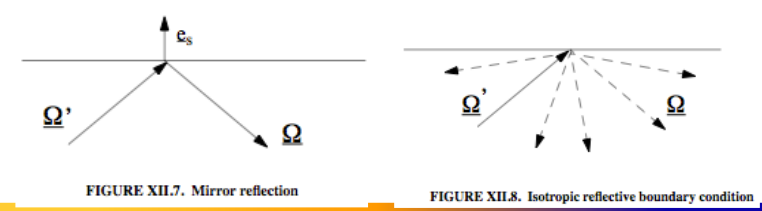
\includegraphics[keepaspectratio, width = 3.5 in]{reflecting-bc}
     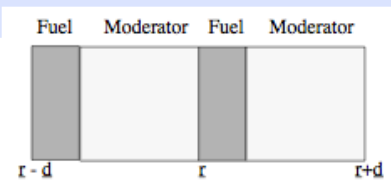
\includegraphics[keepaspectratio, width = 2 in]{periodic-bc}
    \end{center}
\end{figure}


\end{document}
